\documentclass{standalone}
\usepackage[T1]{fontenc}
\usepackage[latin2]{inputenc}
\usepackage[english]{babel}
\usepackage{caption}
\usepackage{graphicx}
\usepackage{tikz}
\usepackage{times}
\usetikzlibrary{calc,through,backgrounds,positioning,fit}
\usetikzlibrary{shapes,arrows,shadows}
\usepackage{boxhandler}
\usepackage{tabularx}

\begin{document}
\begin{tikzpicture}
\node (n1)[label=above:{\textsl{Data with cluster assigned}}] [stt] at (-3.5,0) {
\begin{table}
\begin{tabular}{|c|c|c|c|c||c|}
\hline
 $t$&$a_{1}$&$a_{2}$&\dots &$a_{k}$&$c$\\ \hline \hline
 $t_{1}$&$v_{1}^{1}$&$v_{2}^{1}$&\dots &$v_{k}^{1}$&$c_{1}$ \\ \hline
 $t_{2}$&$v_{1}^{2}$&$v_{2}^{2}$&\dots &$v_{k}^{2}$&$c_{2}$ \\ \hline
 \dots & \dots &\dots &\dots &\dots &\dots\\ \hline
 $t_{n}$&$v_{1}^{n}$&$v_{2}^{n}$&\dots &$v_{k}^{n}$&$c_{n}$ \\ \hline
 \dots & \dots &\dots &\dots &\dots &\dots \\ \hline
\end{tabular}
\end{table}
};

\node (n2)[label=above:{\textsl{State graph}}] [stt] at (3.5,0) {
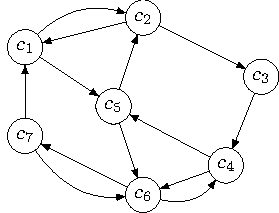
\includegraphics[scale=1]{statesgraph.pdf}
};

\draw [-to,gray,ultra thick] (n1) -- (n2) node[color=black, pos=0.5, above, text width=1.5cm] {\small{Process discovery}}; 

\end{tikzpicture}

\end{document}

